% AP Statistics — Unit 2, Topic 2.5: Correlation
% Minimal teacher-facing comments included per spec.
\documentclass[11pt]{article}
\usepackage[letterpaper,margin=0.9in]{geometry}
\usepackage{enumitem}
\usepackage{multicol}
\usepackage{amsmath,amssymb}
\usepackage{tikz}
\usepackage{pgfplots}
\pgfplotsset{compat=1.18}

\setlist[itemize]{itemsep=0.2em,topsep=0.2em}
\setlist[enumerate]{itemsep=0.35em,topsep=0.35em}

\newcommand{\ts}[1]{\texttt{[#1]}} % timestamp placeholder

\title{AP Statistics\\Unit 2, Topic 2.5: Correlation}
\author{}
\date{}

\begin{document}
\maketitle

\small

\section*{Objectives (DAT-1 aligned)}
% From framework.md: DAT-1, properties of r, Skills 2.C and 4.B
\begin{itemize}
  \item Define correlation $r$ and describe its \textbf{direction} and \textbf{strength} for linear associations.
  \item Recall key properties of $r$: unit-free; $-1\le r \le 1$; $r\approx 0$ implies no \emph{linear} association; $|r|$ near $1$ does not alone justify a linear model.
  \item Skill 2.C: Determine/compute $r$ using technology when appropriate.
  \item Skill 4.B: Interpret $r$ in context using correct statistical language.
  \item Distinguish correlation from causation; recognize potential third variables (lurking variables).
\end{itemize}

\section*{Follow-Along Prompts (with timestamps)}
% Timestamps sourced from u2l5/transcript.txt
\begin{enumerate}[leftmargin=*]
  \item \ts{02:04} Write a concise definition of the correlation coefficient $r$.\\\rule{\linewidth}{0.6pt}
  \item \ts{03:03} What does the \emph{sign} of $r$ tell you? What does the \emph{magnitude} of $r$ tell you?\\\rule{\linewidth}{0.6pt}
  \item \ts{02:41} List two properties of $r$ that are always true.\\\rule{\linewidth}{0.6pt}
  \item \ts{03:16} If $r=0$, what can and can’t we conclude about the relationship?\\\rule{\linewidth}{0.6pt}
  \item \ts{05:39} When might a \emph{large} $|r|$ still not justify a linear model? Give a quick sketch or explanation.\\\rule{\linewidth}{0.6pt}
  \item \ts{04:53} \textbf{Correlation vs. Causation:} Give an example of a third (lurking) variable that could explain an observed correlation.\\\rule{\linewidth}{0.6pt}
  \item \ts{02:24} Technology check (Skill 2.C): In your calculator or software, where do you find $r$ for a scatterplot/regression output?\\\rule{\linewidth}{0.6pt}
  \item \ts{03:51} Interpretation (Skill 4.B): In words, interpret $r= -0.62$ for a linear association in a reasonable context.\\\rule{\linewidth}{0.6pt}
\end{enumerate}

\vspace{0.6em}
\section*{Mini-Activity: Estimate $r$ from Micro-Plots}
\noindent \textit{For each plot A--C, estimate $r$ (direction and magnitude). Explain your reasoning in a few words.}

\begin{center}
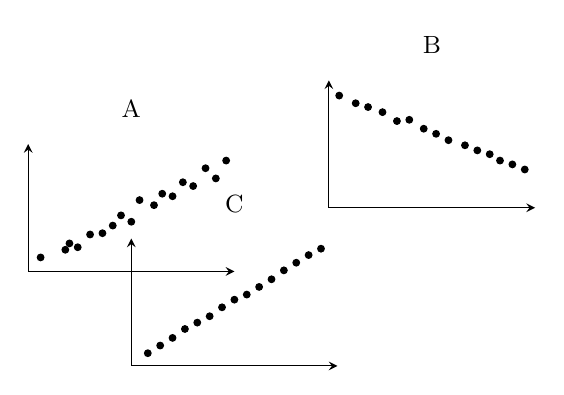
\begin{tikzpicture}[scale=1]
  % Micro-plot A: weak positive (r ~ +0.25)
  \begin{axis}[
    name=plotA,
    width=4.2cm,height=3.2cm,
    xmin=0,xmax=10,ymin=0,ymax=10,
    axis lines=left, ticks=none,
    title={\small A}
  ]
    \addplot[only marks, mark=*, mark size=1.2pt] table[row sep=\\]{
      x y\\
      0.6 1.1\\ 1.8 1.7\\ 2.0 2.2\\ 2.4 1.9\\ 3.0 2.9\\ 3.6 3.0\\ 4.1 3.6\\ 4.5 4.4\\ 5.0 3.9\\ 5.4 5.6\\
      6.1 5.2\\ 6.5 6.1\\ 7.0 5.9\\ 7.5 7.0\\ 8.0 6.7\\ 8.6 8.1\\ 9.1 7.3\\ 9.6 8.7\\
    };
  \end{axis}

  % Micro-plot B: medium negative (r ~ -0.60)
  \begin{axis}[
    at={(plotA.east)}, xshift=1.2cm,
    width=4.2cm,height=3.2cm,
    xmin=0,xmax=10,ymin=0,ymax=10,
    axis lines=left, ticks=none,
    title={\small B}
  ]
    \addplot[only marks, mark=*, mark size=1.2pt] table[row sep=\\]{
      x y\\
      0.5 8.8\\ 1.3 8.2\\ 1.9 7.9\\ 2.6 7.5\\ 3.3 6.8\\ 3.9 6.9\\ 4.6 6.2\\ 5.2 5.8\\ 5.8 5.3\\ 6.6 4.9\\
      7.2 4.5\\ 7.8 4.2\\ 8.3 3.7\\ 8.9 3.4\\ 9.5 3.0\\
    };
  \end{axis}

  % Micro-plot C: strong positive (r ~ +0.90)
  \begin{axis}[
    at={(plotA.south)}, yshift=-1.2cm,
    width=4.2cm,height=3.2cm,
    xmin=0,xmax=10,ymin=0,ymax=10,
    axis lines=left, ticks=none,
    title={\small C}
  ]
    \addplot[only marks, mark=*, mark size=1.2pt] table[row sep=\\]{
      x y\\
      0.8 1.0\\ 1.4 1.6\\ 2.0 2.2\\ 2.6 2.9\\ 3.2 3.4\\ 3.8 3.9\\ 4.4 4.6\\ 5.0 5.2\\ 5.6 5.6\\ 6.2 6.2\\
      6.8 6.8\\ 7.4 7.5\\ 8.0 8.1\\ 8.6 8.7\\ 9.2 9.2\\
    };
  \end{axis}
\end{tikzpicture}
\end{center}

\vspace{0.2em}
\noindent\textbf{Your estimates:}\quad A: $r\approx$ \rule{1.6cm}{0.4pt}\quad B: $r\approx$ \rule{1.6cm}{0.4pt}\quad C: $r\approx$ \rule{1.6cm}{0.4pt}

\section*{Reflection: Attendance vs Scores}
% Per spec: tie to the attendance↑ vs scores flat question.
\noindent A school reports rising class attendance while average test scores remain roughly flat.\newline
\textbf{Prompt:} What does this suggest about the correlation between attendance and scores? Could a third variable explain both?\\\rule{\linewidth}{0.6pt}

\vspace{0.6em}
\section*{Quick Checks}
\begin{multicols}{2}
\begin{enumerate}[leftmargin=*]
  \item True/False: $r$ is measured in the same units as the variables.\\\rule{\linewidth}{0.4pt}
  \item Circle one: If $r=0.80$, the association is (weak / moderate / strong) and (positive / negative).\\\rule{\linewidth}{0.4pt}
  \item Does $r=0$ prove “no relationship” between two variables? Explain briefly.\\\rule{\linewidth}{0.4pt}
  \item Name one reason a linear model might be inappropriate even when $|r|$ is near 1.\\\rule{\linewidth}{0.4pt}
\end{enumerate}
\end{multicols}

\newpage
\section*{Answer Key (Compact)}
% Keep compact to fit 1–2 pages.
\begin{itemize}
  \item Def.: $r$ quantifies \emph{direction} and \emph{strength} of a \textbf{linear} association between two quantitative variables.
  \item Properties: unit-free; $-1\le r\le 1$; $r\approx 0$ means no linear association; $|r|\approx 1$ does not by itself justify linear modeling.
  \item Sign vs magnitude: sign gives direction (positive/negative); $|r|$ gives strength (closer to 1 is stronger).
  \item $r=0$: no linear association; there may still be non-linear patterns.
  \item Large $|r|$ but poor linear fit: e.g., outliers leverage $r$; curved relationships; heteroscedasticity.
  \item Lurking variable example: rain drives both umbrella sales and accidents; neither causes the other.
  \item Mini-activity (one reasonable set): A $\approx +0.25$ (weak +), B $\approx -0.60$ (medium −), C $\approx +0.90$ (strong +).
  \item Attendance vs scores: likely small/near-zero correlation overall; a third variable (e.g., instructional changes, assessment difficulty) may influence both.
  \item Quick checks: (1) False. (2) strong, positive. (3) No—only no \emph{linear} relationship. (4) Outliers/curvature/unequal spread.
\end{itemize}

% Teacher note: Replace \ts{mm:ss} with accurate timestamps once transcript is available.

\end{document}
